\documentclass[12pt]{article}

\usepackage[margin=1in]{geometry}
\geometry{lettersize}

\usepackage{graphicx}
\usepackage{float}
\usepackage{wrapfig}
\usepackage{caption}
\usepackage{hyperref}
\usepackage{subcaption}

\linespread{1.2}

\renewcommand{\maketitle}{
    \begin{flushright}
        {\LARGE \textbf{Randomization in Path Planning}}


    {\large \textsc{Wenhan Zhu (Cosmos)} \\ \textit{University of Waterloo}}
    \\ \today

    \end{flushright}
}

\begin{document}

\maketitle

\section*{Introduction}
Many path planning algorithms rely on randomness for fast calculation. In many situations, calculating the optimal path is not feasible or time consuming. So many algorithms focuses on generating a path quickly and if possible improving the path generated when time allows. Rapidly-exploring random tree (RRT)\cite{LaValle1998} is one of these algorithms. This report discusses about RRT and another popular path planning algorithm Probabilistic Roadmap (PRM) \cite{Kavraki1996}. And at the end also focuses on the improvements on RRT and some open ideas on the topic.

\section*{Motivation}
My previous research focuses on path planning for autonomous vehicles. In particular the path planning aspect in local planner. The local planner plans the exact vehicle path to navigate on the road. It generates an exact path that the vehicle needs to follow and a corresponding speed profile that guides the controller. As part of the autonomous driving software it needs to run updates in very short intervals and requires the path to be executable by the vehicle. Many research has been conducted in this area, but there are still no dominating solution when the scenario is complex. This is mainly due to dynamic objects and the unpredictable behaviours of human operated vehicles on the road. I've come across RRT when I was studying animations and AI in games. It turns out that RRT was originally designed to solve the problem of motion planning for robotics. Which is highly related to the field of autonomous vehicles. However, many other problem still remain unsolved for such approach. More details are discussed in the later sections of this report.

\section*{PRM and RRT}
Both PRM and RRT are introduced in the late 90s to solve the problem of having a continuous state space and obstacles that needs to be avoided, how to generate a path between a start state and end state in the state spaces. They both assume the obstacles are convex, but in practice they also works well in many situations when the obstacles are not convex. Many applications of both the algorithms and it's variant are used in practice. A brief overview of both the algorithms are discussed in the following sections. 

\begin{figure}
\centering
\begin{subfigure}{.5\textwidth}
    \centering
    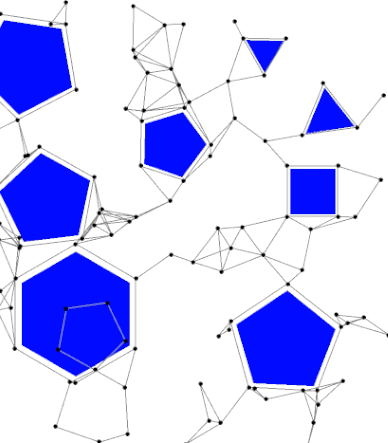
\includegraphics[width=.6\linewidth]{prm-example.png}
    \caption{PRM example (Source: Wiki)}
    \label{fig:prm}
\end{minipage}%
\begin{subfigure}{.5\textwidth}
    \centering
    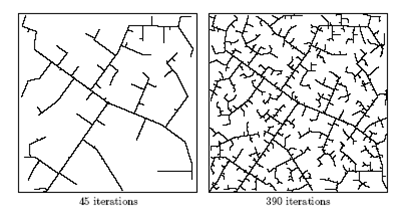
\includegraphics[width=.6\linewidth]{rrt-example.png}
    \caption{RRT example (Source: Wiki)}
    \label{fig:rrt}
\end{minipage}
\caption{PRM and RRT example}
\end{figure}



\subsection*{PRM}
In principle, PRM creates a set of points as a boundary for each obstacle in the space. Then it adds random points in the space and connects points that are with in a range and does not cross over obstacles. After adding many points so that the graph is connected, we can then use search algorithms such as A* on the graph to calculate the shortest path.

\subsection*{RRT}
As its name, RRT expands a tree with a root at the starting state and randomly sample from the space and connect the sample to the closest node on the existing tree if a feasible connection can be found. Once we are able to connect the goal to the tree, we can track back the nodes of the tree from where it is connected to the root. 

\subsection*{Comparison}
From the design of these two algorithms, we can see that they have a lot of difference which makes one more useful in certain situations than the other. Here, let us compare some of the differences and how it affects applications.

PRM consists of two phases, first construction and then search. So it's really useful in situations where we only need to construct the graph once and then search multiple times. For example, in RTS (Real-time strategy) games, many adopt a navigation mesh that represents this idea and then do shortest path search when we need to find a path between to points. RRT on the other hand does not have this property, it constructs the tree and also the path in the same time. Which means that every time we need to find the path between two points we need to run the algorithm again. However, RRT also doesn't need any preprocessing as PRM. So base on application we might prefer one to the other. 

\section*{Randomization in Path Planning}
In the execution of PRM and RRT, there are two parts that heavily uses randomization. 

\subsection*{Sampling}
Both PRM and RRT use sampling in the space to find solutions. In their original introduction, they are both based on uniform sampling. With uniform sampling, the number of points that needed to cover the space can be calculated using ideas of balls and bins and Voronoi diagrams. For a simple example, if we want every point in the space to be connect in PRM, with preprocessing of the obstacles, we only need enough points to cover the entire graph with a tessellation distance the same as the radius we decided to connect between two points. 

\subsection*{Nearest Neighbor}
When constructing the graph, we need to connect points to their nearest neighbor in both the algorithms. While in low dimensions, kd-trees performs nicely, it's often not the case in higher dimensions. Randomized algorithms such as randomized kd-tree provides great performance improvements in such situations. However, in my previous area of research it was not a main concern.

\section*{Limitations}
PRM and RRT provides a path between two points. However, neither of them is able to provide a path that converges to the optimal path nicely. PRM is able to converge to the optimal path, but the number of points needed to is too large which increases the searching time dramatically. Research has shown that RRT does not converge to the optimal path \cite{Karaman2010}. But a adaption of RRT called optimal RRT (RRT*) will converge to the optimal path and converges quickly. The details is shown in the next section.

Another limitation is the smoothness of the path generated. PRM by design is a discrete graph and therefore it can't generate a path that's smooth. RRT on the other hand is able to provide a smooth path based on the agents movement, however, the result is often very jerky and does not provide a smooth path in second or higher orders. Which means in the application of autonomous vehicles, the vehicle will be very uncomfortable. 

\section*{Improvements of RRT}
As previously mentioned, RRT* is an adaptation of RRT that's able to converge to the optimal path and preserve many nice properties of RRT.

Compared to RRT, in RRT* when a new vertex is added to the tree, it optimizes the edges in the collection of the tree by evaluating the cost of adding the new vertex and it's related edges. With this added step, the path generated to each point will not deviate from the optimal path too much. Karaman et. al. showed that the convergence rate of such algorithm is $\log{n}$ which is very nice.

\section*{Open problems and ideas}
PRM and RRT focuses on generating a path between 2 points. RRT can solve the path finding problem for a nonholonomic robot. However, in the application of autonomous vehicles they do not take some other important factors into consideration. One of these is the comfort of driving. The main factor that affects the comfort is the jerk. In the previous section, we discussed why neither of these methods can generate a low jerk path. More actions like smoothing are needed to provide a nice smooth path, however, such steps often take much more computing time and is not idea in practice. 

Another important factor is velocity considerations in autonomous driving. When a path is generated by RRT, the model can't easily integrate the change of velocity in the vehicle. When the speed of the vehicle changes, the possible maneuver the vehicle is able to perform also changes. Therefore, in practice, more dynamic models of RRT needs to be used but often the computing time of such algorithms are very expensive. 

\section*{Conclusion}
Randomization plays a huge role in many path planning algorithms. PRM, RRT and their variants are very important in the field. Many improvements are still being introduced from time to time. I'm very curious to see what improvements they will receive in the future. 

\section*{Acknowledgements}
Some description of PRM and RRT came from a undergrad project I worked on with Zixiao Wang. More details can be found here: \href{https://cosmos-graphics.github.io/projects/project_3/index.html}{Fall 2015 CSCI 5611 Project 3} It's nice to actually read the original papers and thinking about some analysis on these algorithm compared to only implementing them back when I was an undergrad.





\bibliographystyle{alpha}

\bibliography{sample}

\end{document}
